%%%%%%%%%%%%%%%%%%%%%%%%%%%%%%%%%%%%%%%%%%%%%%%%%%%%%%%%%%%%
% INSTRUCTIONS:
% This section may be divided by subheadings. Footnotes should not be used and must be transferred to the main text.
%%%%%%%%%%%%%%%%%%%%%%%%%%%%%%%%%%%%%%%%%%%%%%%%%%%%%%%%%%%%

\section{Results}

\subsection{Adaptive phenotypic plasticity slows evolutionary change in fluctuating environments}


\begin{figure}[h!]
    \centering
    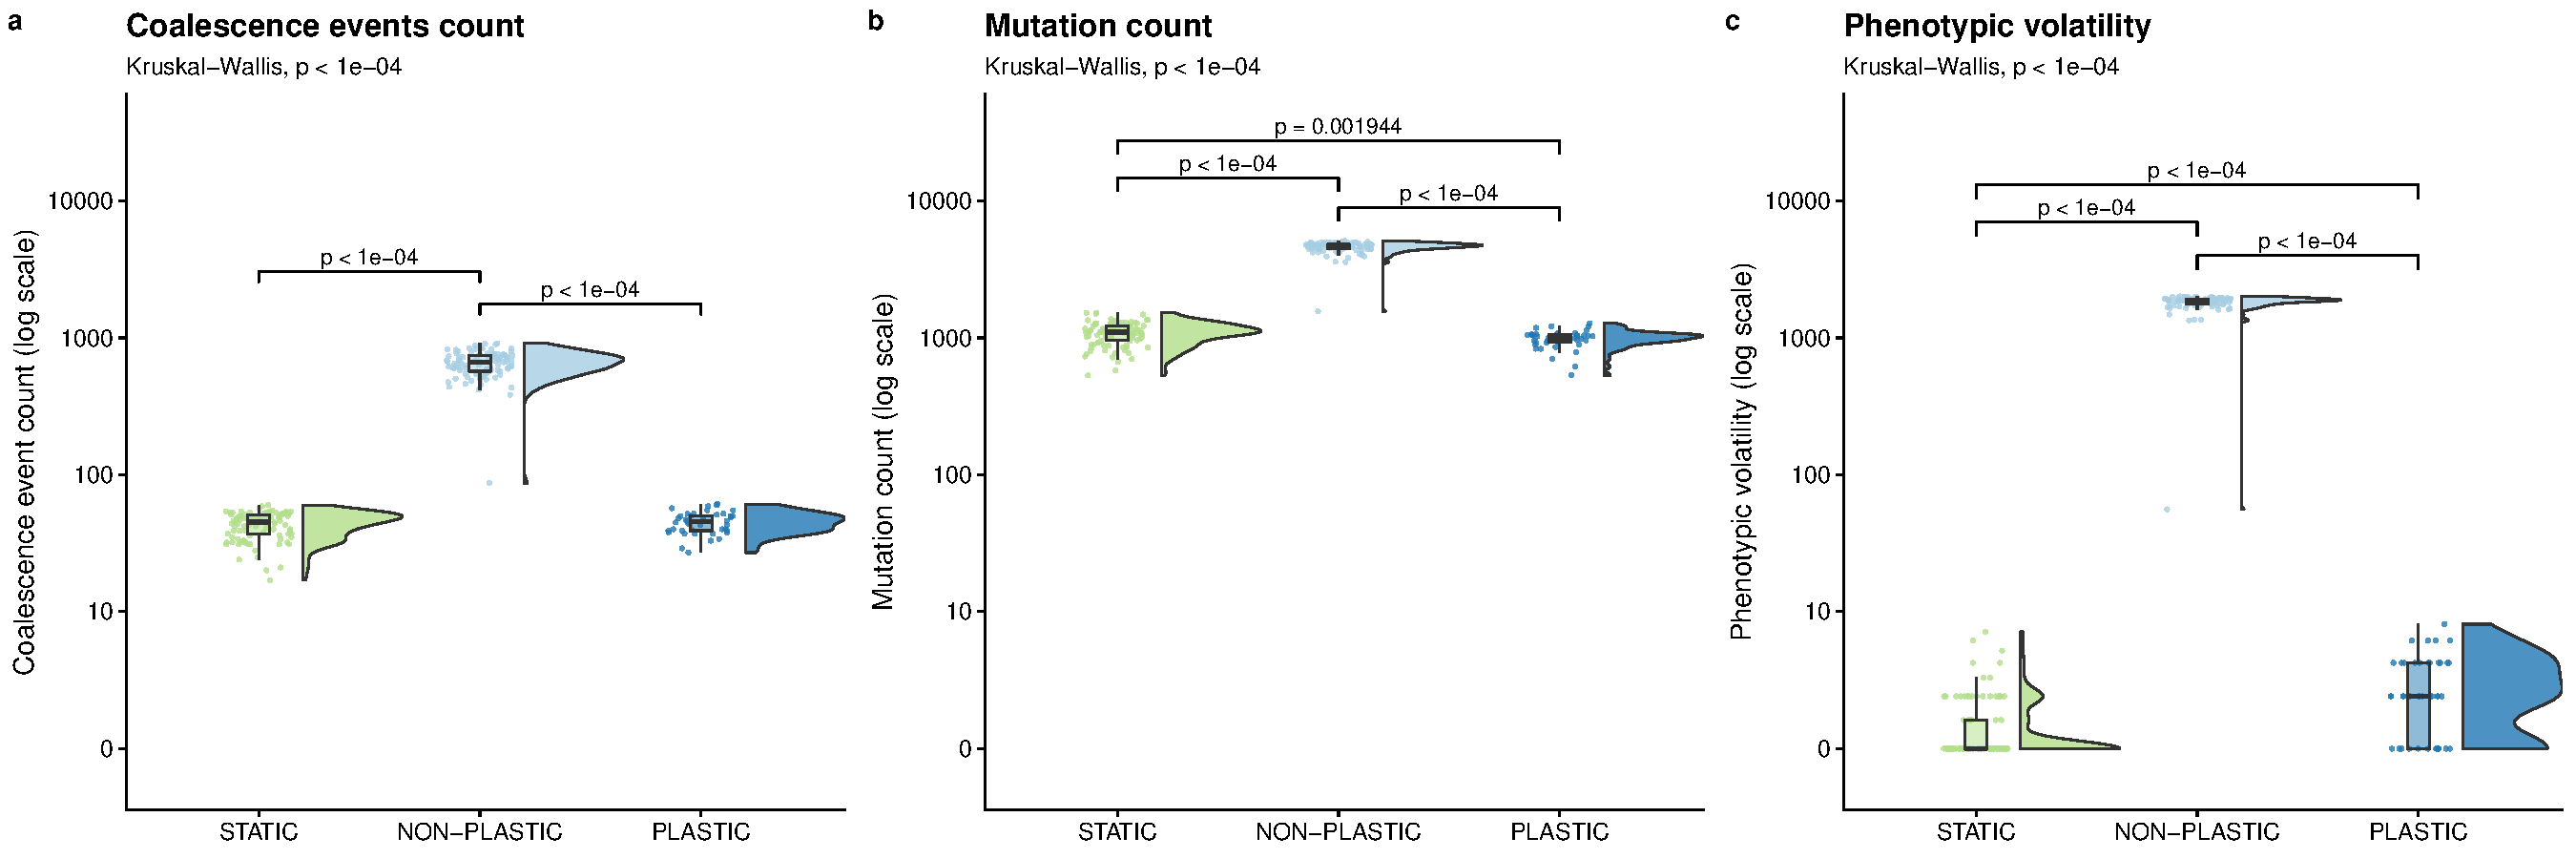
\includegraphics[width=1\textwidth]{media-evolutionary-change-magnitude-panel.pdf}
    \caption{\small
    \textbf{Magnitude of evolutionary change.}
    Raincloud plots \citep{allen_raincloud_2019} of
    (a) coalescence event count,
    (b) mutation count,
    and (c) phenotypic volatility.
    See Table \ref{tab:metrics-definitions} for descriptions of each metric.
    Each plot is annotated with statistically significant comparisons (Bonferroni-corrected pairwise Wilcoxon rank-sum tests).
    Note that adaptive phenotypic plasticity evolved in \evolutionaryChangeRatePlasticReps\ of \evolutionaryChangeRateReplicates\ replicates from the PLASTIC treatment during phase one of this experiment; we used this more limited group to found \evolutionaryChangeRatePlasticReps\ phase-two PLASTIC replicates from which we report these PLASTIC data.
    }
    \label{fig:evolutionary-dynamics-magnitude}
\end{figure}


%%%%%%%%%%%%%%%%%%%%%%%%%%%%%%%%%
% Results to report (2021-02-08 experiment)
% ----- GENERATIONS -----
% - average generations elapsed (of a population)
%   - NON-PLASTIC (median: 41768.65) > PLASTIC (median: 31697.65) > STATIC (median: 30839.75)
%   condition     mean    sd
%   <chr>        <dbl> <dbl>
% 1 NON-PLASTIC 41090. 2702.
% 2 PLASTIC     31016. 2615.
% 3 STATIC      30002. 3011.

%
% ----- SWEEPS -----
% - coalescence events (total)
%   - NON-PLASTIC (median: 663.5) > ( PLASTIC (median: 45.5) ~~ STATIC (median: 45) )
% - Average number of generations between coalescence events (gens / sweeps)
%   - ( PLASTIC (median: 685.001780758557) ~~ STATIC (median: 693.676265008576) ) > NON-PLASTIC (median: 62.0184902295191)
%
% ----- PHENOTYPIC VOLATILITY -----
% - phenotypic volatility (total)
%   - i.e., total number of times phenotypes change along lineages
%   - NON-PLASTIC (median: 1868) > PLASTIC (median: 2) > STATIC (median: 0)
% - phenotypic volatility / lineage length
%   - i.e., how often do genomic changes reflect changes in phenotype?
%   - NON-PLASTIC (median: 0.437) > PLASTIC (median: 0.0022) > STATIC (median: 0)
% - phenotypic volatility / generations
%   - i.e., per-offspring rate of phenotypic changes
%   - NON-PLASTIC (median: 0.0447) > PLASTIC (median: 6.33e-05) > STATIC (median: 0)
%
% ----- MUTATION ACCUMULATION -----
% - mutation accumulation (total)
%   - NON-PLASTIC (median: 4657.5) > STATIC (median: 1100) > PLASTIC (median: 998.5)
% - mutation accumulation / lineage length
%   - NON-PLASTIC (median: 1.10048311715591) > STATIC (median: 1.03794597464116) > PLASTIC (median: 1.0328599144651)
% - mutation accumulation / generation
%   - NON-PLASTIC (median: 0.11) > STATIC (median: 0.0368) > PLASTIC (median: 0.0319)
%
% ----- MUTATIONAL EFFECTS -----
% - fraction of mutational steps that alter (aggregate) phenotype
%   - NON-PLASTIC (mean: 0.434007, CI [0.4242,  0.4406]) > PLASTIC (mean: 0.002717008, 0.0020,  0.0035) > STATIC (mean: 0.0006788834, CI [0.0004,  0.0009])
% - fraction of phenotype-altering mutation steps that alter unexpressed phenotype (PLASTIC condition only)
%   - mean: 0.8247126 CI [0.7443,  0.8994]
% - fraction of mutations that affect unexpressed phenotype that are deleterious (PLASTIC only)
%   - mean: 0.5172414 CI [0.4402,  0.5977]
% - fraction of mutations that affect unexpressed phenotype that are beneficial (PLASTIC only)
%   - mean: 0.4827586 CI [0.4046,  0.5598]
%%%%%%%%%%%%%%%%%%%%%%%%%%%%%%%%%

% -- Magnitude of evolutionary change --
%  - Selective sweeps
%  - Mutation accumulation
%  - Phenotypic volatility
In experimental phase 2A,
we tested whether adaptive phenotypic plasticity constrained or promoted subsequent evolutionary change in a fluctuating environment.
First, we compared the total amount of evolutionary change in populations evolved under the PLASTIC, NON-PLASTIC, and STATIC treatments as measured by coalescence event count, mutation count, and phenotypic volatility (Figure \ref{fig:evolutionary-dynamics-magnitude}).
According to each of these metrics, NON-PLASTIC populations experienced a larger magnitude of evolutionary change than either PLASTIC or STATIC populations.
We observed significantly higher coalescence event counts in NON-PLASTIC populations than in PLASTIC or STATIC populations (Figure \ref{fig:evolutionary-dynamics-magnitude}\hyperref[fig:evolutionary-dynamics-magnitude]{a}).
NON-PLASTIC lineages had significantly higher mutation counts (Figure \ref{fig:evolutionary-dynamics-magnitude}b) and phenotypic volatility than PLASTIC or STATIC lineages (Figure \ref{fig:evolutionary-dynamics-magnitude}c).

% -- Elapsed generations --
Changing environments have been shown to increase generational turnover in Avida populations \citep{canino-koning_evolution_2016}, which could explain why we observe a larger magnitude of evolutionary change at the end of 200,000 updates of evolution in NON-PLASTIC populations.
Indeed, we found that significantly more generations of evolution elapsed in NON-PLASTIC populations (mean of $41090\pm2702$ std. dev.) than in PLASTIC (mean of $31016\pm2615$ std. dev.) or STATIC (mean of $30002\pm3011$ std. dev.) populations during phase 2A (corrected Wilcoxon rank-sum tests, p $<10^{-4}$).

% -- Rate of evolutionary change => intuition --
To evaluate whether increased generational turnover explains the greater magnitude of evolutionary change in NON-PLASTIC populations, we examined the average number of generations between coalescence events and the realized mutational robustness of lineages (Table \ref{tab:metrics-definitions}).
A coalescence event indicates a selective sweep, which is a hallmark of adaptive evolutionary change.
Realized mutational robustness measures the frequency that mutations cause phenotypic changes along a lineage.
We expect that static conditions should favor fit lineages with high realized mutational robustness that no longer undergo rapid adaptive change and hence do not trigger frequent coalescence events.
Under fluctuating conditions, however, lineages must be composed of plastic organisms if they are to maintain both high fitness and realized mutational robustness.
Without plasticity, we expect fluctuating conditions to produce lineages with low realized mutational robustness and frequent coalescence events as populations must continually acquire and fix mutations to readapt to the environment.


\begin{figure}[h!]
    \centering
    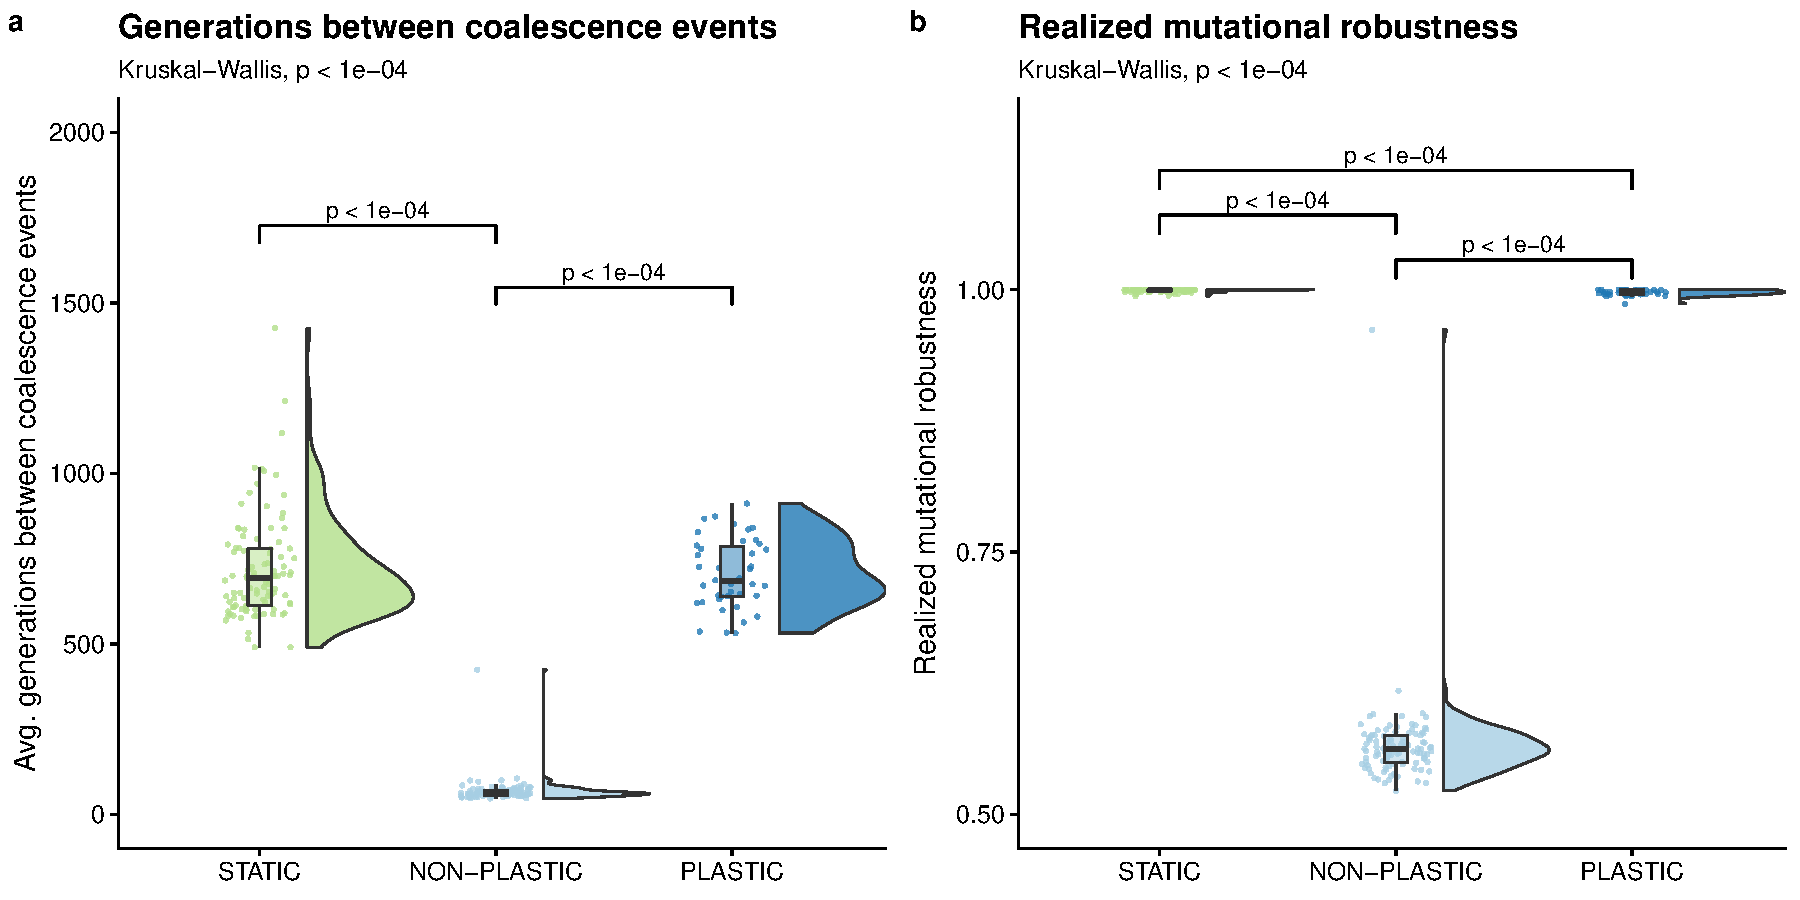
\includegraphics[width=0.66\textwidth]{media-evolutionary-change-pace-panel.pdf}
    \caption{\small
    \textbf{Pace of evolutionary change.}
    Raincloud plots of
    (a) average number of generations between coalescence events,
    and (b) realized mutational robustness (Table \ref{tab:metrics-definitions}).
    Each plot is annotated with statistically significant comparisons (Bonferroni-corrected pairwise Wilcoxon rank-sum tests).
    }
    \label{fig:evolutionary-dynamics-rate}
\end{figure}

% -- Rate of evolutionary change => findings --
On average, significantly fewer generations elapsed between coalescence events in NON-PLASTIC populations than in either PLASTIC or STATIC populations (Figure \ref{fig:evolutionary-dynamics-rate}a).
We also found that both STATIC and PLASTIC lineages exhibited higher realized mutational robustness relative to that of NON-PLASTIC lineages (Figure \ref{fig:evolutionary-dynamics-rate}b); that is, mutations observed along NON-PLASTIC lineages more often caused phenotypic changes in offspring.
Overall, our results indicate that NON-PLASTIC populations underwent more rapid (and thus a greater amount of) evolutionary change than either PLASTIC or STATIC populations.

% -- Mutational stability in static and plastic lineages --
While both STATIC and PLASTIC lineages exhibited high realized mutational robustness, we found that STATIC lineages exhibited higher realized robustness than PLASTIC lineages (Figure \ref{fig:evolutionary-dynamics-rate}b).
Overall, there were rare instances of mutations that caused a change in phenotypic profile across all PLASTIC lineages.
Of these mutations, we found that over 80\% (83 out of 102) of changes to phenotypic profiles were cryptic.
That is, the mutations affected traits that would not have been expressed in the environment that the organism was born into but would have been expressed had the environment changed.

\begin{figure}[ht!]
    \centering
    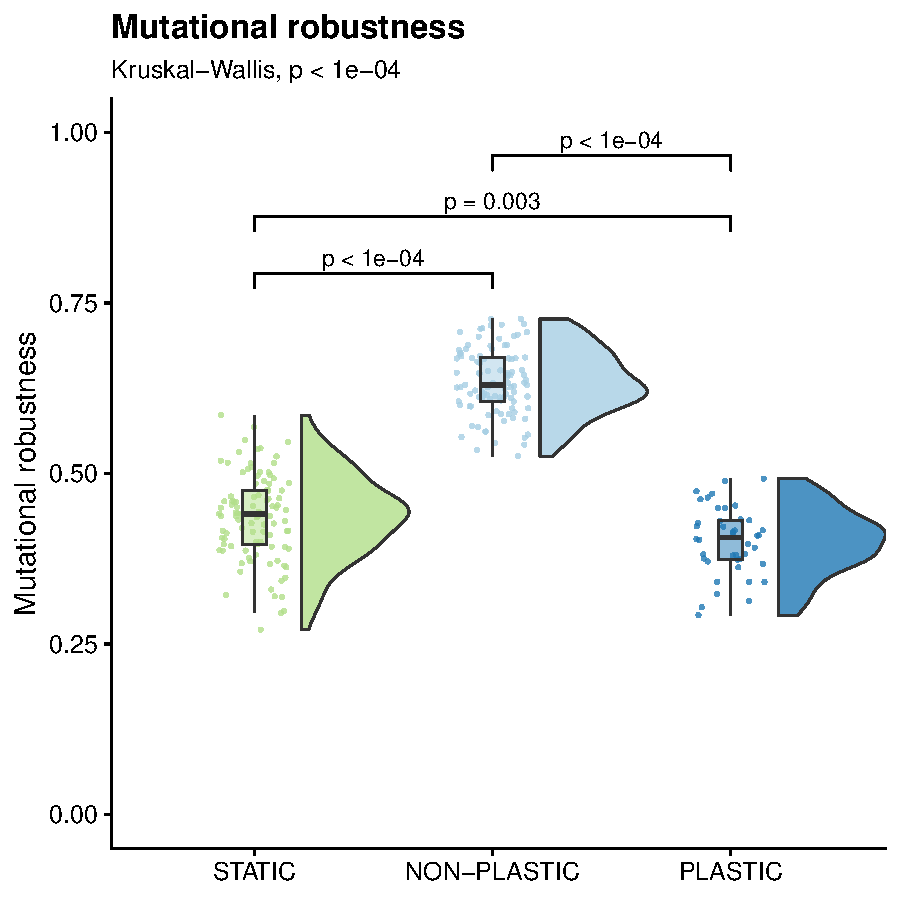
\includegraphics[width=0.33\textwidth]{media-mutational-robustness.pdf}
    \caption{\small
        \textbf{Mutational robustness.}
        Raincloud plot of mutational robustness of each representative genotype (Table \ref{tab:metrics-definitions}).
        The plot is annotated with statistically significant comparisons (Bonferroni-corrected pairwise Wilcoxon rank-sum tests).
    }
    \label{fig:mutational-robustness}
\end{figure}

% -- mutational landscaping --
% Thus far, our analyses have focused on dominant lineage.
% What about mutations off the line of descent?
% Mutational stability result is NOT due to random mutations being more likely to induce phenotypic change.
% KEY: Motivation for looking at mutational neighborhoods needs to made very clear here
%   - Why not look at mutational neighborhoods for the other experiments?
Given that NON-PLASTIC lineages exhibited the lowest realized mutational robustness of our three experimental treatments, we sought to determine if this effect was driven by differences in evolved genetic architectures.
Specifically, did the NON-PLASTIC genetic architectures evolve such that mutations were more likely to result in phenotypic change?
Such a  mutational bias would trade off descendant fitness in the same environment in exchange for a chance of increasing descendant fitness in alternate environments.
This strategy would be an example of diversifying bet-hedging (\textit{i.e.}, reducing expected mean fitness to lower variance in fitness) \citep{childs2010evolutionary}.
Alternatively, the lower realized mutational robustness in NON-PLASTIC lineages could be due to survivorship bias, as we measured realized mutational robustness as the fraction of mutations observed along \textit{successful} lineages that caused a phenotypic change.
%(\textit{i.e.}, the lineages of extant organisms)


We analyzed the mutational robustness of representative genotypes by calculating the fraction of single-instruction mutations that change the phenotypic profile.
We found that mutations to representative genotypes on NON-PLASTIC lineages are \textit{less} likely to result in a phenotypic change than mutations to comparable genotypes on either STATIC or PLASTIC lineages (Figure \ref{fig:mutational-robustness}).
These data provide evidence against NON-PLASTIC lineages engaging in a mutation-driven bet-hedging strategy, and instead, are consistent with the hypothesis that lower realized mutational robustness in the NON-PLASTIC treatment was due to survivorship bias.
% @AML: Maybe one more sentence elaborating on implication of survivorship bias?

% -- in general, PLASTIC and STATIC more similar than NON-PLASTIC --
In general, adaptive plasticity stabilized PLASTIC-treatment populations against environmental fluctuations, and their evolutionary dynamics more closely resembled those of populations evolving in a static environment.
We observed no significant difference in the number and frequency of coalescence events in PLASTIC and STATIC populations.
We did, however, observe small, but statistically significant, differences in each of the following metrics: elapsed generations, mutation counts, mutational robustness, and realized mutational robustness between PLASTIC and STATIC populations.

\vspace{0.5cm}
\subsection{Adaptively plastic populations retain more novel tasks than non-plastic populations in fluctuating environments}

%%%%%%%%%%%%%%%%%%%%%%%%%%%%%%%%%
% Results to report (2021-01-31)
% - Number of plastic replicates
% - Final dominant genotype # novel traits
%   - non-plastic < (plastic == static)
% - Final population (1% threshold):
%   - non-plastic < plastic < static
% - Final population (1% threshold) discovered:
%   - non-plastic > (plastic ~~ static)
% - Lineage tasks discovered
%   - non-plastic > static ~>(nosig) plastic
% - Lineage tasks discovered / step
%   - (static ~~ plastic) > non-plastic
% - Lineage tasks lost
%   - non-plastic > static > plastic
% - Lineage tasks lost / step
%   - non-plastic > static > plastic

% - tasks discovered per generation(?)
%   - NON-PLASTIC [0.00014358046266055] ~~ STATIC [0.00015363220504867] > PLASTIC [0.000117695011124939]
% - tasks lost per generation(?)
%   - NON-PLASTIC [0.0022026054610079] > STATIC [0.000161396283669756] > PLASTIC [6.25141973661864e-05]
%%%%%%%%%%%%%%%%%%%%%%%%%%%%%%%%%

\begin{figure}[h!]
    \centering
    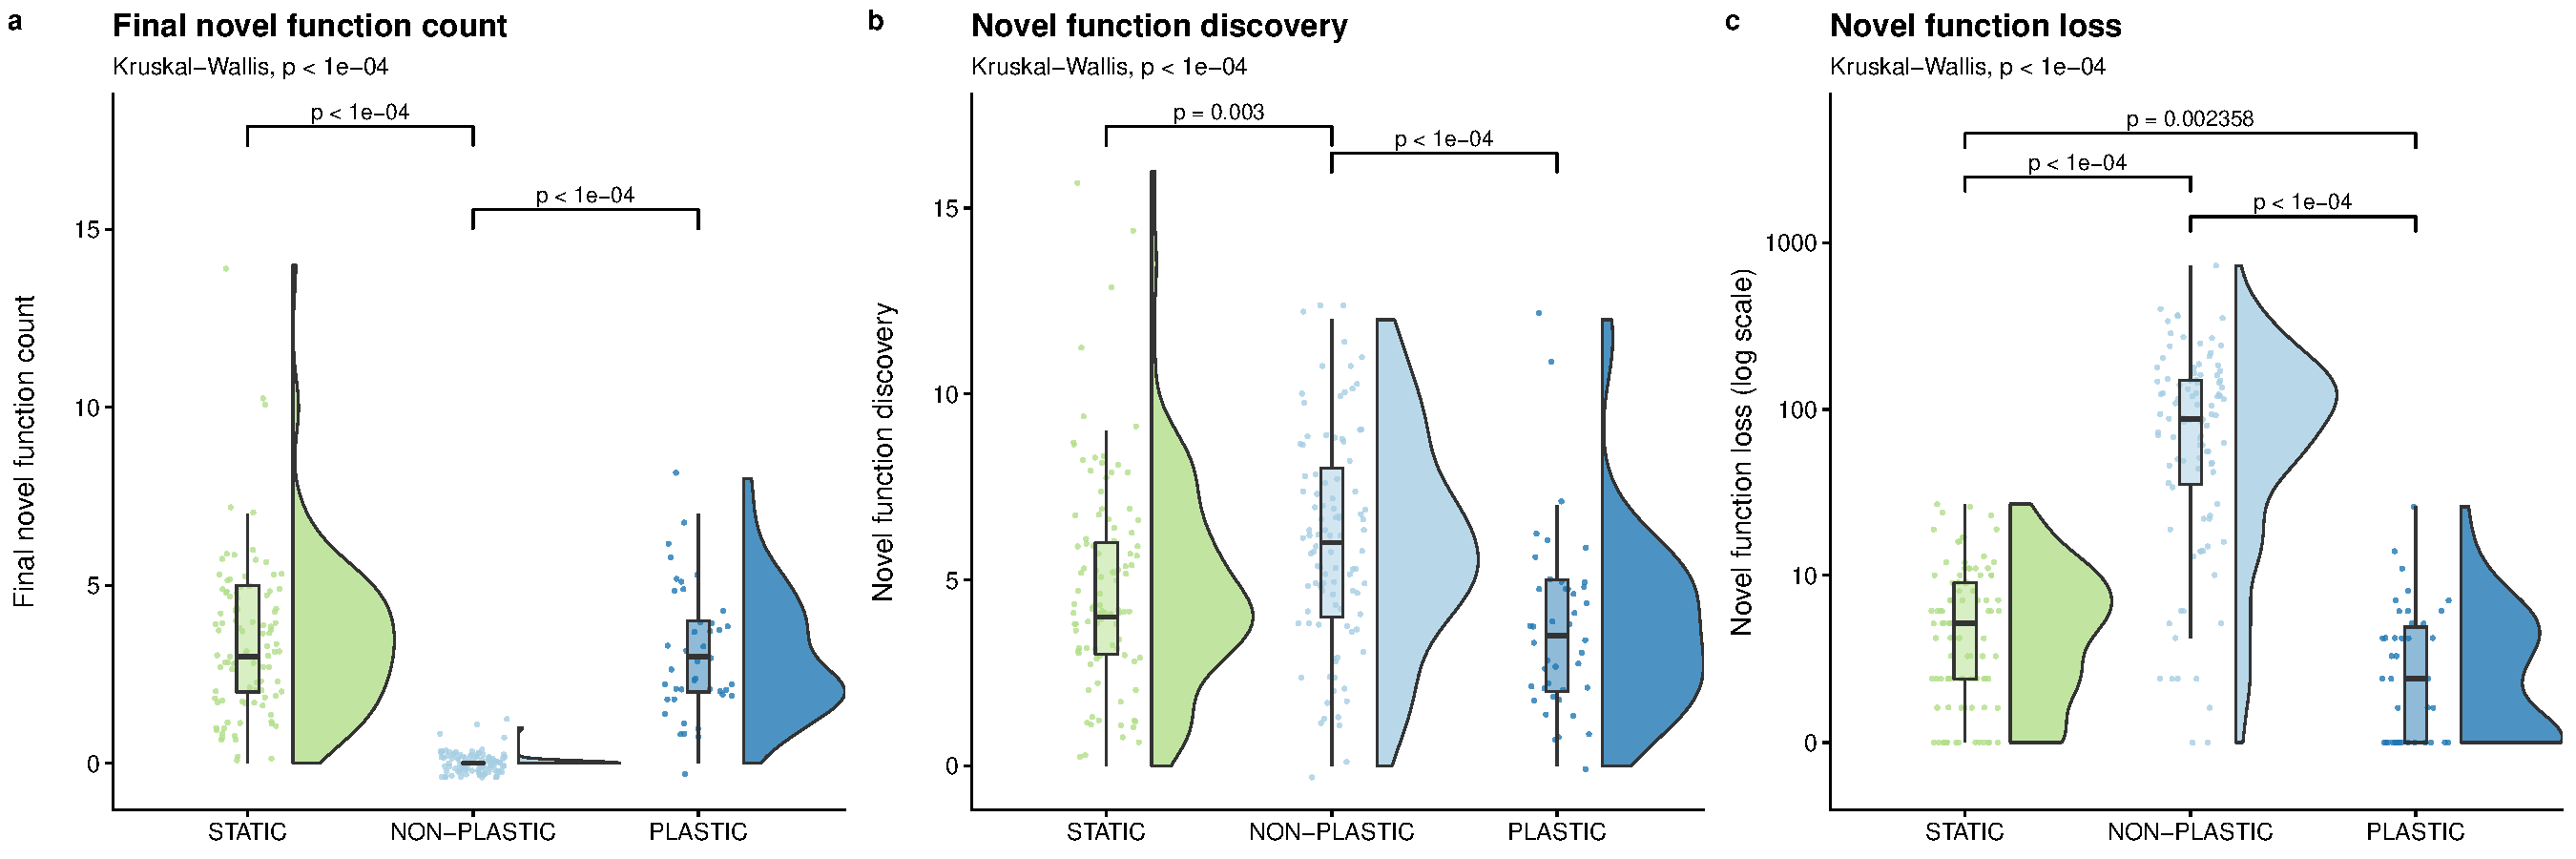
\includegraphics[width=0.9\textwidth]{media-complex-traits-magnitude-panel.pdf}
    \caption{\small
    \textbf{Novel task evolution.}
    Raincloud plots of
    (a) final novel task count,
    (b) novel task discovery,
    and (c) novel task loss.
    See Table \ref{tab:metrics-definitions} for descriptions of each metric.
    Each plot is annotated with statistically significant comparisons (Bonferroni-corrected pairwise Wilcoxon rank-sum tests).
    Note that adaptive phenotypic plasticity evolved in \novelTraitsPlasticReps\ of \novelTraitsReplicates\ replicates from the PLASTIC treatment during phase one of this experiment; we used this more limited group to seed the resulting \novelTraitsPlasticReps\ phase-two PLASTIC replicates.
    }
    \label{fig:complex-traits-magnitude}
\end{figure}

% -- What did we test? --
%In experimental phase 2B, we evaluated how evolution of adaptive phenotypic plasticity influences the ability of populations to evolve and retain novel adaptive traits. Commented out by Nkrumah...
We have so far shown that adaptive plasticity constrains the rate of evolutionary change in fluctuating environments.
However, it is unclear how this dynamic influences the evolution of novel tasks.
Based on their relative rates of evolutionary change, we might expect NON-PLASTIC-treatment populations to evolve more novel tasks than PLASTIC-treatment populations.
But, how much of the evolutionary change in NON-PLASTIC populations is useful for exploring novel regions of the fitness landscape versus continually rediscovering the same regions?

% - Magnitude of exploration/exploitation -
To answer this question, we quantified the number of novel tasks performed by a representative organism in the final population of each replicate.
We found that both PLASTIC and STATIC populations had significantly higher final task counts than NON-PLASTIC populations at the end of the experiment (Figure~\ref{fig:complex-traits-magnitude}a).
The final novel task count in PLASTIC and STATIC lineages could be higher than that of the NON-PLASTIC lineages for several non-mutually exclusive reasons.
One possibility is that PLASTIC and STATIC lineages could be exploring a larger area of the fitness landscape when compared to NON-PLASTIC lineages.
Another possibility is that the propensity of the NON-PLASTIC lineages to maintain novel traits could be significantly lower than PLASTIC or STATIC lineages.
When we looked at the total sum of novel tasks discovered by each of the PLASTIC, STATIC, and NON-PLASTIC lineages, we found that NON-PLASTIC lineages generally explored a larger area of the fitness landscape (Figure~\ref{fig:complex-traits-magnitude}b).
Although the NON-PLASTIC lineages discovered more novel tasks, those lineages also exhibited significantly higher novel task loss when compared to PLASTIC and STATIC lineages (Figure~\ref{fig:complex-traits-magnitude}c).

\begin{figure}[h!]
    \centering
    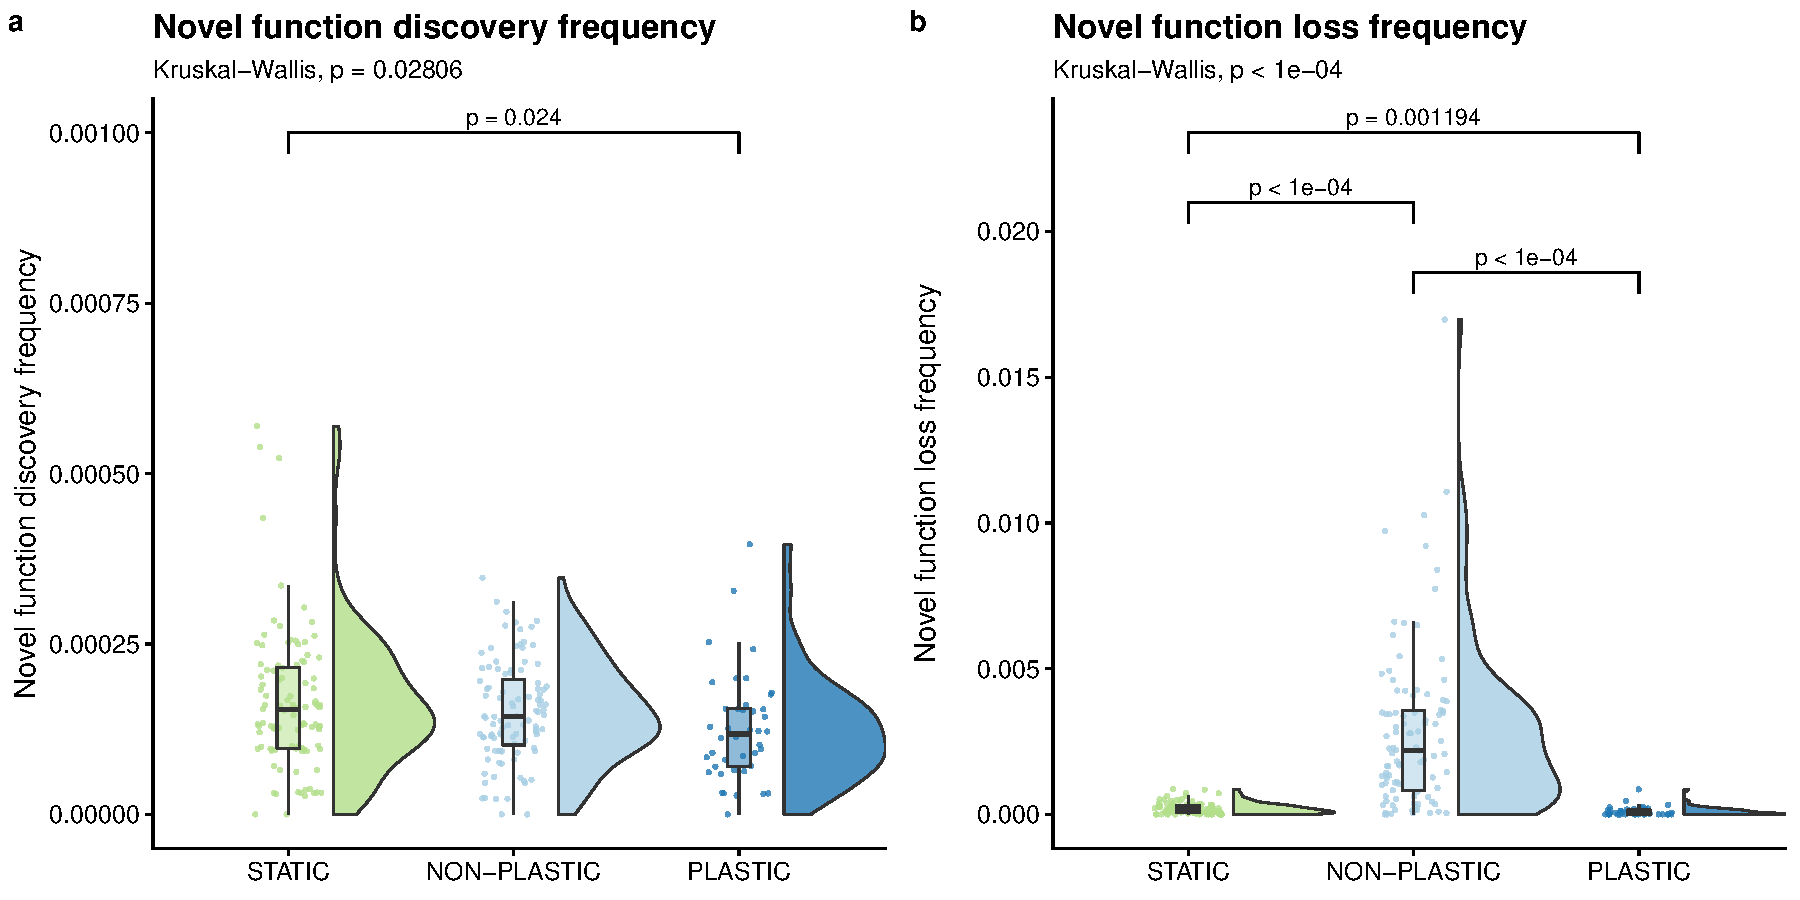
\includegraphics[width=0.66\textwidth]{media-complex-traits-pace-panel.pdf}
    \caption{\small
    \textbf{Rate of novel task evolution.}
    Raincloud plots of
    (a) novel task discovery frequency
    and (b) novel task loss frequency.
    Each plot is annotated with statistically significant comparisons (Bonferroni-corrected pairwise Wilcoxon rank-sum tests).
    }
    \label{fig:complex-traits-rate}
\end{figure}

% - Rates of exploration/exploitation -
A larger number of generations elapsed in NON-PLASTIC populations than in PLASTIC or STATIC populations during our experiment \citep{supplemental_material}.
Are NON-PLASTIC lineages discovering and losing novel tasks more frequently than PLASTIC or STATIC lineages, or are our observations a result of differences in generational turnover?
To answer this question, we converted the metrics of novel task discovery and novel task loss to rates by dividing each metric by the number of elapsed generations along the associated representative lineages.
We found no significant difference in the frequency of novel task discovery between NON-PLASTIC and STATIC lineages, and we found that PLASTIC lineages had a lower frequency of novel task discovery than STATIC lineages (Figure~\ref{fig:complex-traits-rate}a).
Therefore, we cannot reject the possibility that the larger magnitude of task discovery in NON-PLASTIC lineages was driven by a larger number of elapsed generations.
NON-PLASTIC lineages had a higher frequency of task loss than either PLASTIC or STATIC lineages, and PLASTIC lineages tended to have a lower frequency of novel task loss than STATIC lineages (Figure~\ref{fig:complex-traits-rate}b).


% - Characterizing trait loss -
Next, we examined the frequency at which novel task loss along lineages co-occurred with the loss or gain of any of the six base tasks.
Across all NON-PLASTIC representative lineages, over 97\% (10998 out of 11229) of instances of novel task loss co-occurred with a simultaneous change in base task profile.
In contrast, across all PLASTIC and STATIC dominant lineages, we observed that approximately 20\% (29 out of 142) and 2\% (13 out of 631), respectively, of instances of novel task loss co-occurred with a simultaneous change in base task profile.
As such, the losses of novel tasks in NON-PLASTIC lineages appear to be primarily due to hitchhiking.

\subsection{Lineages without plasticity that evolve in fluctuating environments express more deleterious tasks}

%%%%%%
% 2021-02-05 - Results
% - Number of offspring on lineage where hitchhiker instruction execution increases (i.e., instances of hitchhiking)
%   - PLASTIC ~~ STATIC < NON-PLASTIC
% - Hitchhiker instruction increases / offspring on lineage
%   - PLASTIC ~~ STATIC < NON-PLASTIC
% - What fraction of mutations that increase hitchhiker instruction execution co-occur with base trait changes?
%   - NON-PLASTIC > PLASTIC ~~ STATIC
% - What about unexpressed vs expressed trait changes in plastic populations? (plastic only)
%   - Not much hitchhiking. Did not find evidence that hitchiking occurring as cryptic variation in unexpressed phenotype.
%%%%%%

Phenotypic plasticity allows for genetic variation to accumulate in genomic regions that are unexpressed, which could lead to the fixation of deleterious instructions in PLASTIC populations.
However, in NON-PLASTIC lineages, we observe a higher rate of novel task loss, indicating that they may be more susceptible to deleterious mutations (Figure \ref{fig:complex-traits-rate}b).

Therefore, in experiment phase 2C, we tested whether adaptive phenotypic plasticity can increase the incidence of deleterious task performance.
Specifically, we added an instruction that triggered a ``poisonous'' task and measured the number of times it was executed.
Each execution of the  \code{poison} instruction reduces an organism's fitness by 10\%.
At the beginning of phase 2C, the \code{poison} instruction is not present in the population, as it was not part of the instruction set during phase one of evolution.
Accordingly, if a \code{poison} instruction fixes in a population, it must be the result of evolutionary dynamics during phase 2C, including cryptic variation or hitchhiking.

\begin{figure}[ht!]
    \centering
    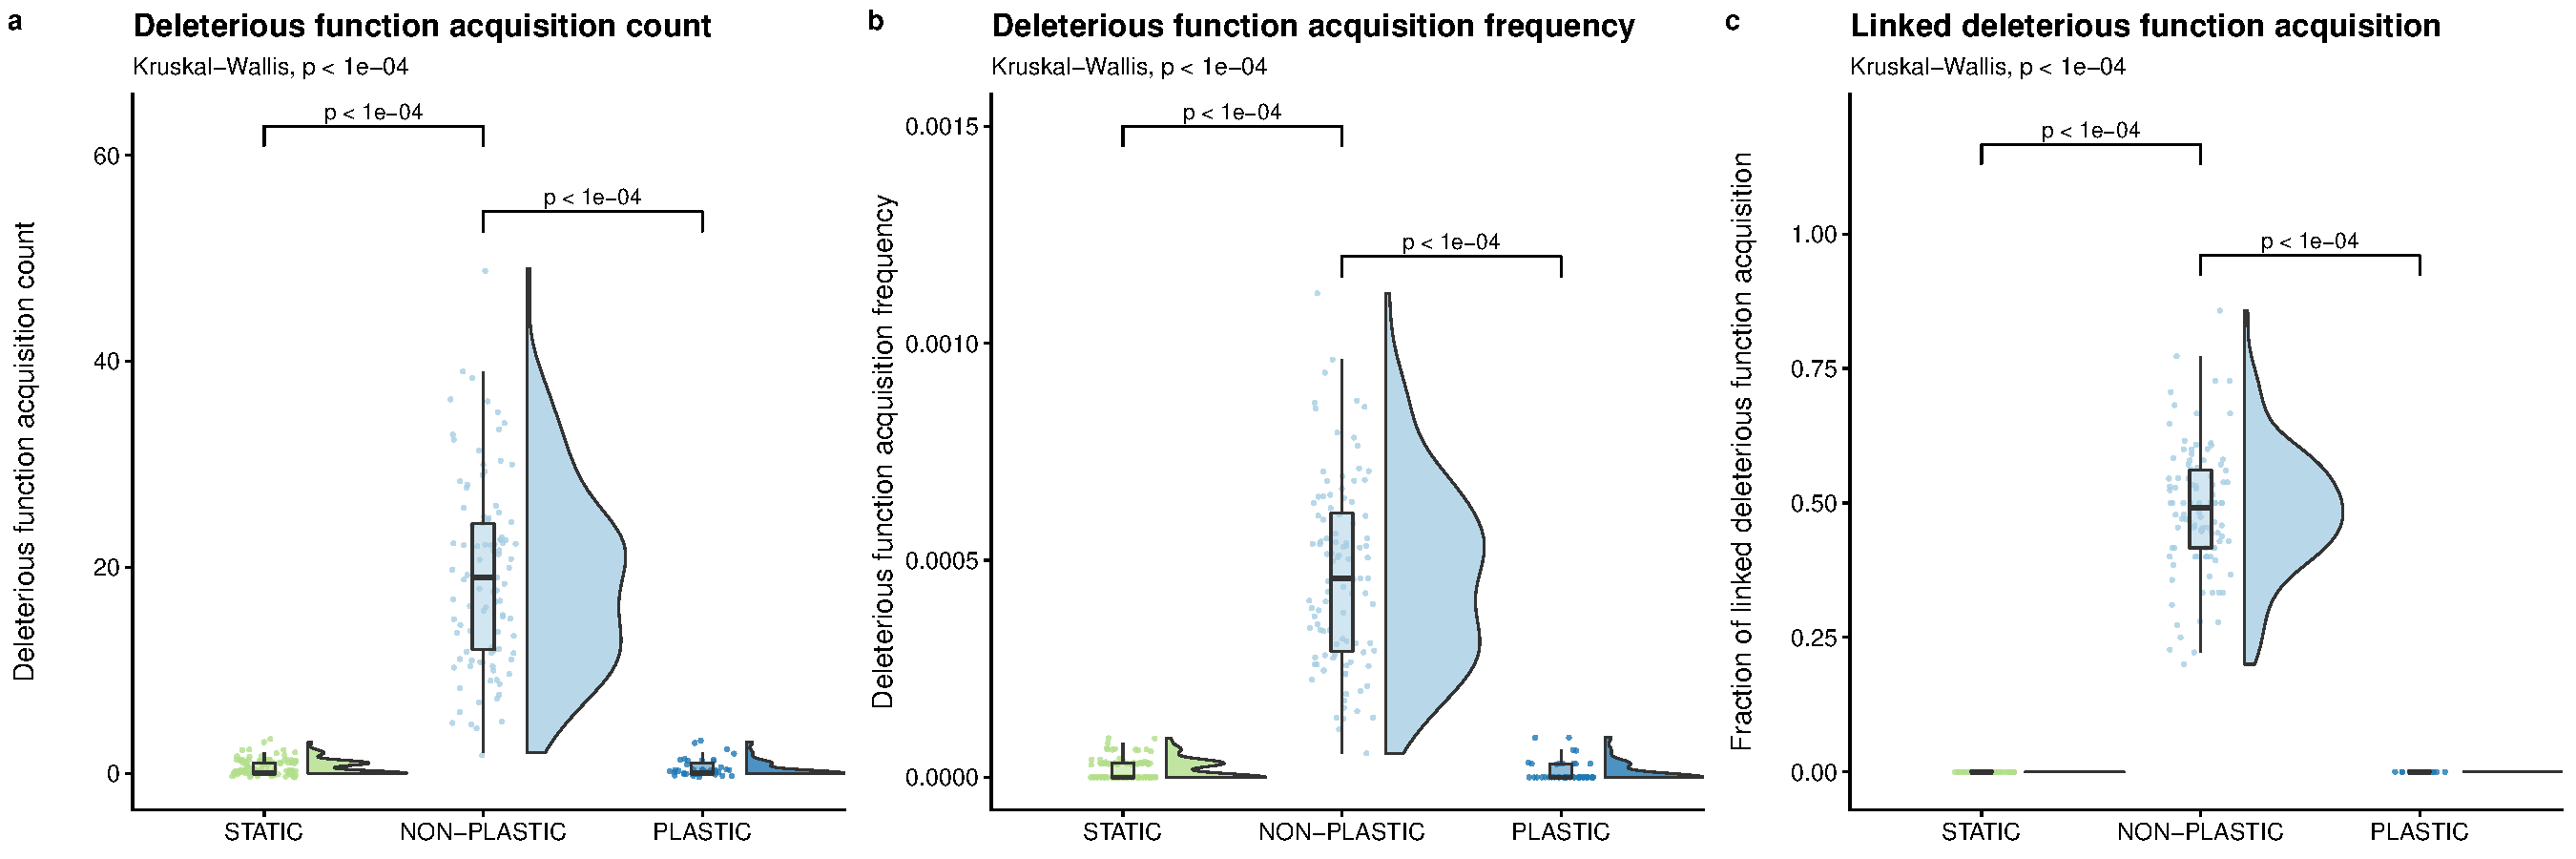
\includegraphics[width=1.0\textwidth]{media-poison-accumulation-panel.pdf}
    \caption{\small
    \textbf{Deleterious instruction accumulation.}
    Raincloud plots of
    (a) poisonous task acquisition,
    (b) poisonous task acquisition frequency,
    and (c) the proportion of mutations that increase poisonous task performance along a lineage that co-occur with a change in phenotypic profile.
    Each plot is annotated with statistically significant comparisons (Bonferroni-corrected pairwise Wilcoxon rank-sum tests).
    Note that adaptive phenotypic plasticity evolved in \deleteriousHitchhikingPlasticReps\ of \deleteriousHitchhikingReplicates\ replicates from the PLASTIC treatment during phase one of this experiment; we used this more limited group to seed the \deleteriousHitchhikingPlasticReps\ phase-two PLASTIC replicates.
    }
    \label{fig:deleterious-hitchhiking}
\end{figure}

% -- Instruction execution by final dominant & along lineage --
At the end of our experiment, no representative organisms from the PLASTIC or STATIC treatments performed the poisonous task under any environmental condition; however, representative organisms in 14\% of replicates of the NON-PLASTIC treatment performed the poisonous task at least once.
NON-PLASTIC lineages contained significantly more mutations that conferred the poisonous task as compared to PLASTIC or STATIC lineages (Figure \ref{fig:deleterious-hitchhiking}a), and these mutations occurred at a significantly higher frequency in NON-PLASTIC lineages (Figure \ref{fig:deleterious-hitchhiking}b).
% Additionally, we did not observe
% This result does not change when we normalize [what?] by the number of generations represented in the given lineage (Figure \ref{fig:deleterious-hitchhiking}b).

% -- When/where does hitchhiking take place? --
Next, we measured how often mutations that increased poisonous task performance co-occurred with changes to the base task profile within representative lineages.
A poisonous instruction can fix in a lineage by having a beneficial effect that outweighs its inherent cost (\textit{e.g.}, knocking out a punished task) or through linkage with a secondary beneficial mutation at another site within the genome.
Across all NON-PLASTIC representative lineages, we found that approximately 49\% (956 out of 1916) of mutations that increased poisonous task expression co-occurred with a change in the base task profile (Figure \ref{fig:deleterious-hitchhiking}c).
In all representative lineages from the PLASTIC treatment, only 18 mutations increased poisonous task expression, and none co-occurred with a change in base task profile (Figure \ref{fig:deleterious-hitchhiking}c).
Likewise, only 58 mutations increased poisonous task performance in all representative lineages from the STATIC treatment, and none co-occurred with a change in base task profile (Figure \ref{fig:deleterious-hitchhiking}c).
We did not find compelling evidence that the few mutations that increased poisonous task expression occurred as cryptic variation in PLASTIC lineages.

We repeated this experiment with 3\% and 30\% metabolic rate penalties associated with the poisonous task, which produced results that were consistent with those reported here \citep{supplemental_material}.